\documentclass[twoside]{book}

% Packages required by doxygen
\usepackage{calc}
\usepackage{doxygen}
\usepackage{graphicx}
\usepackage[utf8]{inputenc}
\usepackage{makeidx}
\usepackage{multicol}
\usepackage{multirow}
\usepackage{textcomp}
\usepackage[table]{xcolor}

% Font selection
\usepackage[T1]{fontenc}
\usepackage{mathptmx}
\usepackage[scaled=.90]{helvet}
\usepackage{courier}
\usepackage{amssymb}
\usepackage{sectsty}
\renewcommand{\familydefault}{\sfdefault}
\allsectionsfont{%
  \fontseries{bc}\selectfont%
  \color{darkgray}%
}
\renewcommand{\DoxyLabelFont}{%
  \fontseries{bc}\selectfont%
  \color{darkgray}%
}

% Page & text layout
\usepackage{geometry}
\geometry{%
  a4paper,%
  top=2.5cm,%
  bottom=2.5cm,%
  left=2.5cm,%
  right=2.5cm%
}
\tolerance=750
\hfuzz=15pt
\hbadness=750
\setlength{\emergencystretch}{15pt}
\setlength{\parindent}{0cm}
\setlength{\parskip}{0.2cm}
\makeatletter
\renewcommand{\paragraph}{%
  \@startsection{paragraph}{4}{0ex}{-1.0ex}{1.0ex}{%
    \normalfont\normalsize\bfseries\SS@parafont%
  }%
}
\renewcommand{\subparagraph}{%
  \@startsection{subparagraph}{5}{0ex}{-1.0ex}{1.0ex}{%
    \normalfont\normalsize\bfseries\SS@subparafont%
  }%
}
\makeatother

% Headers & footers
\usepackage{fancyhdr}
\pagestyle{fancyplain}
\fancyhead[LE]{\fancyplain{}{\bfseries\thepage}}
\fancyhead[CE]{\fancyplain{}{}}
\fancyhead[RE]{\fancyplain{}{\bfseries\leftmark}}
\fancyhead[LO]{\fancyplain{}{\bfseries\rightmark}}
\fancyhead[CO]{\fancyplain{}{}}
\fancyhead[RO]{\fancyplain{}{\bfseries\thepage}}
\fancyfoot[LE]{\fancyplain{}{}}
\fancyfoot[CE]{\fancyplain{}{}}
\fancyfoot[RE]{\fancyplain{}{\bfseries\scriptsize Generated on Tue Mar 14 2017 12\-:05\-:20 for V\-M\-C by Doxygen }}
\fancyfoot[LO]{\fancyplain{}{\bfseries\scriptsize Generated on Tue Mar 14 2017 12\-:05\-:20 for V\-M\-C by Doxygen }}
\fancyfoot[CO]{\fancyplain{}{}}
\fancyfoot[RO]{\fancyplain{}{}}
\renewcommand{\footrulewidth}{0.4pt}
\renewcommand{\chaptermark}[1]{%
  \markboth{#1}{}%
}
\renewcommand{\sectionmark}[1]{%
  \markright{\thesection\ #1}%
}

% Indices & bibliography
\usepackage{natbib}
\usepackage[titles]{tocloft}
\setcounter{tocdepth}{3}
\setcounter{secnumdepth}{5}
\makeindex

% Hyperlinks (required, but should be loaded last)
\usepackage{ifpdf}
\ifpdf
  \usepackage[pdftex,pagebackref=true]{hyperref}
\else
  \usepackage[ps2pdf,pagebackref=true]{hyperref}
\fi
\hypersetup{%
  colorlinks=true,%
  linkcolor=blue,%
  citecolor=blue,%
  unicode%
}

% Custom commands
\newcommand{\clearemptydoublepage}{%
  \newpage{\pagestyle{empty}\cleardoublepage}%
}


%===== C O N T E N T S =====

\begin{document}

% Titlepage & ToC
\hypersetup{pageanchor=false}
\pagenumbering{roman}
\begin{titlepage}
\vspace*{7cm}
\begin{center}%
{\Large V\-M\-C }\\
\vspace*{1cm}
{\large Generated by Doxygen 1.8.6}\\
\vspace*{0.5cm}
{\small Tue Mar 14 2017 12:05:20}\\
\end{center}
\end{titlepage}
\clearemptydoublepage
\tableofcontents
\clearemptydoublepage
\pagenumbering{arabic}
\hypersetup{pageanchor=true}

%--- Begin generated contents ---
\chapter{V\-M\-C H\-O\-O\-K\-I\-U\-M}
\label{index}\hypertarget{index}{}\hypertarget{index_intro_sec}{}\section{Introduction}\label{index_intro_sec}

\chapter{File Index}
\section{File List}
Here is a list of all files with brief descriptions\-:\begin{DoxyCompactList}
\item\contentsline{section}{\hyperlink{_hamiltonian_8_c}{Hamiltonian.\-C} }{\pageref{_hamiltonian_8_c}}{}
\end{DoxyCompactList}

\chapter{File Documentation}
\hypertarget{_hamiltonian_8_c}{\section{Hamiltonian.\-C File Reference}
\label{_hamiltonian_8_c}\index{Hamiltonian.\-C@{Hamiltonian.\-C}}
}
{\ttfamily \#include \char`\"{}my\-Random.\-H\char`\"{}}\\*
{\ttfamily \#include $<$fstream$>$}\\*
{\ttfamily \#include $<$time.\-h$>$}\\*
{\ttfamily \#include $<$set$>$}\\*
{\ttfamily \#include $<$iostream$>$}\\*
{\ttfamily \#include $<$stdlib.\-h$>$}\\*
{\ttfamily \#include $<$algorithm$>$}\\*
{\ttfamily \#include $<$vector$>$}\\*
{\ttfamily \#include $<$math.\-h$>$}\\*
{\ttfamily \#include $<$iomanip$>$}\\*
{\ttfamily \#include $<$boost/math/special\-\_\-functions/factorials.\-hpp$>$}\\*
Include dependency graph for Hamiltonian.\-C\-:\nopagebreak
\begin{figure}[H]
\begin{center}
\leavevmode
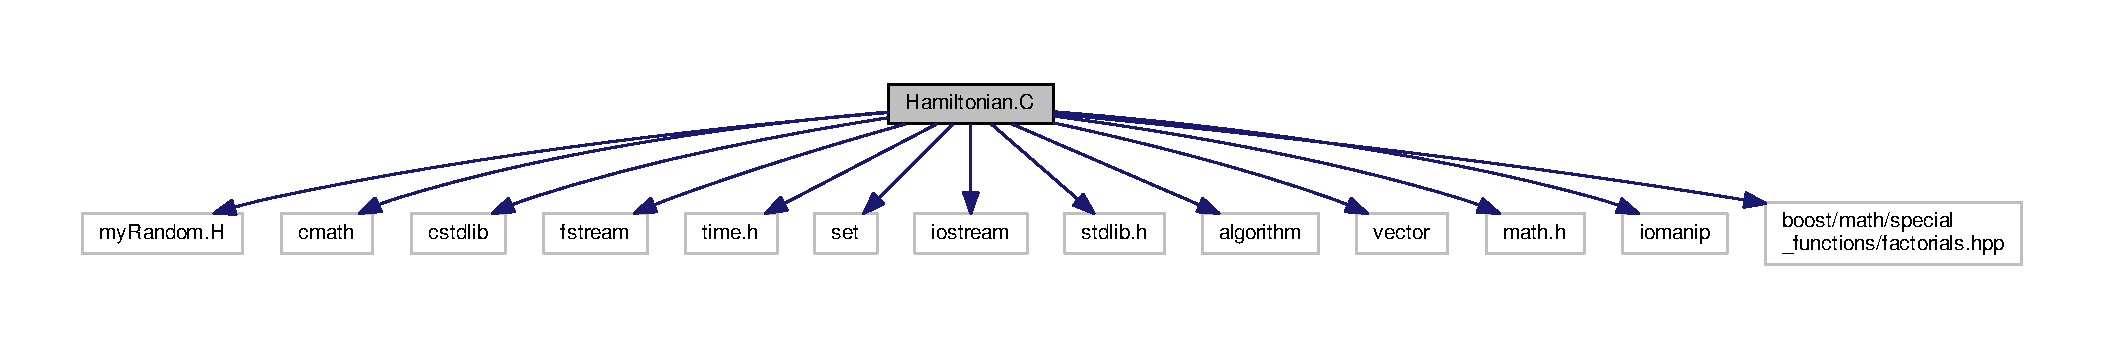
\includegraphics[width=350pt]{_hamiltonian_8_c__incl}
\end{center}
\end{figure}
\subsection*{Functions}
\begin{DoxyCompactItemize}
\item 
double \hyperlink{_hamiltonian_8_c_a99505674b3eaca3ba5e8b87d836b33d3}{hermite\-\_\-\-Nth} (int N, double r)
\item 
double \hyperlink{_hamiltonian_8_c_a7ec5cc277a531db32678aef0ece2f824}{hermite\-\_\-diff1\-\_\-\-Nth} (int N, double r)
\item 
double \hyperlink{_hamiltonian_8_c_a6793465dc0999735fe643355bad66f9c}{hermite\-\_\-diff2\-\_\-\-Nth} (int N, double r)
\item 
double \hyperlink{_hamiltonian_8_c_a55fc72b0d5d57ce3d31669436746fb4c}{beta\-\_\-\-Kth} (int K)
\item 
double \hyperlink{_hamiltonian_8_c_a3d8031037d79fc051beadafd441dcd0c}{Fof\-R\-\_\-\-Kth} (int K, double r)
\item 
double \hyperlink{_hamiltonian_8_c_a19c5936462beaa7be22d387a58f1f3c2}{Fof\-R\-\_\-diff1\-\_\-\-Kth} (int K, double r)
\item 
double \hyperlink{_hamiltonian_8_c_a2529c125e10fca386464e1bb23c81bb7}{Fof\-R\-\_\-diff2\-\_\-\-Kth} (int K, double r)
\item 
double \hyperlink{_hamiltonian_8_c_ae9b5889d7fdd0b64238fdb99de59325a}{P\-H\-I\-\_\-\-Kth} (int K, double r)
\item 
double \hyperlink{_hamiltonian_8_c_acfb28b1644fccbee065d635bd3feae69}{P\-H\-I\-\_\-laplace\-\_\-\-Kth} (int K, double r)
\item 
double \hyperlink{_hamiltonian_8_c_abaf78415afd670c31ce92ab2f4f51a5c}{single\-Particle\-W\-F} (int num\-Terms, double r)
\item 
double \hyperlink{_hamiltonian_8_c_a4f19d549d92d976fea2e9f2a2182dd33}{probabilty\-Weight} (double r1, double r2, double r1\-Trial, double r2\-Trial)
\item 
double \hyperlink{_hamiltonian_8_c_a1ea4c95b4fd14680ab8cce9432ae86ef}{hamiltonian\-Hookium} (int num\-Terms, double r1, double r2)
\item 
double \hyperlink{_hamiltonian_8_c_a1296097286a47b7bb99899a75c931733}{local\-Energy} (int num\-Terms, double r1, double r2)
\item 
int \hyperlink{_hamiltonian_8_c_a840291bc02cba5474a4cb46a9b9566fe}{main} (void)
\end{DoxyCompactItemize}
\subsection*{Variables}
\begin{DoxyCompactItemize}
\item 
const double \hyperlink{_hamiltonian_8_c_a38ea2cbc62615007f27ca01aebdc04a8}{kspring} = 0.\-25
\item 
const double \hyperlink{_hamiltonian_8_c_a0dac55511b8235578f5364bcd618056f}{S\-Q\-R\-T2} = 1.\-4142135623730950488
\item 
const double \hyperlink{_hamiltonian_8_c_a9e3e25918df4dde4f87afaba7778d262}{W\-F\-Coeff} \mbox{[}4\mbox{]} = \{1, 0.\-10825043, -\/0.\-00940132, 0.\-00157574\}
\end{DoxyCompactItemize}


\subsection{Function Documentation}
\hypertarget{_hamiltonian_8_c_a55fc72b0d5d57ce3d31669436746fb4c}{\index{Hamiltonian.\-C@{Hamiltonian.\-C}!beta\-\_\-\-Kth@{beta\-\_\-\-Kth}}
\index{beta\-\_\-\-Kth@{beta\-\_\-\-Kth}!Hamiltonian.C@{Hamiltonian.\-C}}
\subsubsection[{beta\-\_\-\-Kth}]{\setlength{\rightskip}{0pt plus 5cm}double beta\-\_\-\-Kth (
\begin{DoxyParamCaption}
\item[{int}]{K}
\end{DoxyParamCaption}
)}}\label{_hamiltonian_8_c_a55fc72b0d5d57ce3d31669436746fb4c}
This is simply a constant coefficient for f(r), or \char`\"{}\-Fof\-R\-\_\-\-Kth\char`\"{}\-: \[ \beta _k = \frac{ \sqrt{2}}{ 2^k \sqrt{ (2k-1)! } (2\pi)^{ \frac{3}{4} } } \] 

Definition at line 89 of file Hamiltonian.\-C.



Referenced by Fof\-R\-\_\-diff1\-\_\-\-Kth(), Fof\-R\-\_\-diff2\-\_\-\-Kth(), and Fof\-R\-\_\-\-Kth().


\begin{DoxyCode}
89                       \{
90     \textcolor{keywordtype}{double} beta;
91     \textcolor{keywordtype}{double} denom;
92     \textcolor{keywordtype}{double} Kfloat = K;
93     \textcolor{keywordtype}{double} factorial = boost::math::factorial<double>(2*Kfloat - 1);
94     \textcolor{comment}{//std::cout << "FACTORIAL USED = " << factorial << std::endl;}
95     beta = pow(2, 0.5);
96     denom = pow(2, Kfloat) * pow( factorial ,0.5) * pow(2*M\_PI, (3.0/4.0) );
97     beta *= 1/denom;
98     \textcolor{keywordflow}{return} beta;
99 \}
\end{DoxyCode}
\hypertarget{_hamiltonian_8_c_a19c5936462beaa7be22d387a58f1f3c2}{\index{Hamiltonian.\-C@{Hamiltonian.\-C}!Fof\-R\-\_\-diff1\-\_\-\-Kth@{Fof\-R\-\_\-diff1\-\_\-\-Kth}}
\index{Fof\-R\-\_\-diff1\-\_\-\-Kth@{Fof\-R\-\_\-diff1\-\_\-\-Kth}!Hamiltonian.C@{Hamiltonian.\-C}}
\subsubsection[{Fof\-R\-\_\-diff1\-\_\-\-Kth}]{\setlength{\rightskip}{0pt plus 5cm}double Fof\-R\-\_\-diff1\-\_\-\-Kth (
\begin{DoxyParamCaption}
\item[{int}]{K, }
\item[{double}]{r}
\end{DoxyParamCaption}
)}}\label{_hamiltonian_8_c_a19c5936462beaa7be22d387a58f1f3c2}
This function returns the first derivative of $ f_k(r) $, which has the form\-: \[ f'_k(r) = \beta _k \Big\{ \frac{1}{r} H'_{2k-1} (\frac{r}{\sqrt{2}}) - \frac{1}{r^2} H_{2k-1} (\frac{r}{\sqrt{2}}) ) \Big\} \] 

Definition at line 123 of file Hamiltonian.\-C.



References beta\-\_\-\-Kth(), hermite\-\_\-diff1\-\_\-\-Nth(), hermite\-\_\-\-Nth(), and S\-Q\-R\-T2.



Referenced by P\-H\-I\-\_\-laplace\-\_\-\-Kth().


\begin{DoxyCode}
123                                       \{
124     \textcolor{keywordtype}{int} N = 2*K - 1;
125     \textcolor{keywordtype}{double} beta = \hyperlink{_hamiltonian_8_c_a55fc72b0d5d57ce3d31669436746fb4c}{beta\_Kth}(K);
126     \textcolor{keywordtype}{double} hermite\_diff1 = \hyperlink{_hamiltonian_8_c_a7ec5cc277a531db32678aef0ece2f824}{hermite\_diff1\_Nth}(N, (r/\hyperlink{_hamiltonian_8_c_a0dac55511b8235578f5364bcd618056f}{SQRT2}));
127     \textcolor{keywordtype}{double} hermite\_2km1 = \hyperlink{_hamiltonian_8_c_a99505674b3eaca3ba5e8b87d836b33d3}{hermite\_Nth}(N, (r/\hyperlink{_hamiltonian_8_c_a0dac55511b8235578f5364bcd618056f}{SQRT2}));
128     \textcolor{keywordtype}{double} result = (beta/r)*( hermite\_diff1 - (hermite\_2km1/r) );
129     \textcolor{keywordflow}{return} result;
130 \}
\end{DoxyCode}
\hypertarget{_hamiltonian_8_c_a2529c125e10fca386464e1bb23c81bb7}{\index{Hamiltonian.\-C@{Hamiltonian.\-C}!Fof\-R\-\_\-diff2\-\_\-\-Kth@{Fof\-R\-\_\-diff2\-\_\-\-Kth}}
\index{Fof\-R\-\_\-diff2\-\_\-\-Kth@{Fof\-R\-\_\-diff2\-\_\-\-Kth}!Hamiltonian.C@{Hamiltonian.\-C}}
\subsubsection[{Fof\-R\-\_\-diff2\-\_\-\-Kth}]{\setlength{\rightskip}{0pt plus 5cm}double Fof\-R\-\_\-diff2\-\_\-\-Kth (
\begin{DoxyParamCaption}
\item[{int}]{K, }
\item[{double}]{r}
\end{DoxyParamCaption}
)}}\label{_hamiltonian_8_c_a2529c125e10fca386464e1bb23c81bb7}
This function returns the second derivative of $ f_k(r) $, which has the form\-: \[ f''_k(r) = \frac{\beta _k}{r^3} \Big\{ r^2 H''_{2k-1} (\frac{r}{\sqrt{2}}) - 2rH'_{2k-1}(\frac{r}{\sqrt{2}}) + 2H_{2k-1} (\frac{r}{\sqrt{2}}) ) \Big\} \] 

Definition at line 140 of file Hamiltonian.\-C.



References beta\-\_\-\-Kth(), hermite\-\_\-diff1\-\_\-\-Nth(), hermite\-\_\-diff2\-\_\-\-Nth(), hermite\-\_\-\-Nth(), and S\-Q\-R\-T2.



Referenced by P\-H\-I\-\_\-laplace\-\_\-\-Kth().


\begin{DoxyCode}
140                                       \{
141     \textcolor{keywordtype}{int} N = 2*K - 1;
142     \textcolor{keywordtype}{double} beta = \hyperlink{_hamiltonian_8_c_a55fc72b0d5d57ce3d31669436746fb4c}{beta\_Kth}(K);
143     \textcolor{keywordtype}{double} hermite\_2km1 = \hyperlink{_hamiltonian_8_c_a99505674b3eaca3ba5e8b87d836b33d3}{hermite\_Nth}(N, (r/\hyperlink{_hamiltonian_8_c_a0dac55511b8235578f5364bcd618056f}{SQRT2}));
144     \textcolor{keywordtype}{double} hermite\_diff1 = \hyperlink{_hamiltonian_8_c_a7ec5cc277a531db32678aef0ece2f824}{hermite\_diff1\_Nth}(N, (r/\hyperlink{_hamiltonian_8_c_a0dac55511b8235578f5364bcd618056f}{SQRT2}));
145     \textcolor{keywordtype}{double} hermite\_diff2 = \hyperlink{_hamiltonian_8_c_a6793465dc0999735fe643355bad66f9c}{hermite\_diff2\_Nth}(N, (r/\hyperlink{_hamiltonian_8_c_a0dac55511b8235578f5364bcd618056f}{SQRT2}));
146     \textcolor{keywordtype}{double} result = (beta/(r*r*r))*( r*r*hermite\_diff2 - 2*r*hermite\_diff1 + 2*hermite\_2km1 );
147     \textcolor{keywordflow}{return} result;
148 \}
\end{DoxyCode}
\hypertarget{_hamiltonian_8_c_a3d8031037d79fc051beadafd441dcd0c}{\index{Hamiltonian.\-C@{Hamiltonian.\-C}!Fof\-R\-\_\-\-Kth@{Fof\-R\-\_\-\-Kth}}
\index{Fof\-R\-\_\-\-Kth@{Fof\-R\-\_\-\-Kth}!Hamiltonian.C@{Hamiltonian.\-C}}
\subsubsection[{Fof\-R\-\_\-\-Kth}]{\setlength{\rightskip}{0pt plus 5cm}double Fof\-R\-\_\-\-Kth (
\begin{DoxyParamCaption}
\item[{int}]{K, }
\item[{double}]{r}
\end{DoxyParamCaption}
)}}\label{_hamiltonian_8_c_a3d8031037d79fc051beadafd441dcd0c}
This function defines $ f_k(r) $, which is itself a function of $ H_{2k-1}(r), \ \beta _{k} $ \-: \[ f_k (r) = H_{2k-1}( \frac{r}{ \sqrt{2} } ) \frac {\beta _k}{r} \] 

Definition at line 108 of file Hamiltonian.\-C.



References beta\-\_\-\-Kth(), hermite\-\_\-\-Nth(), and S\-Q\-R\-T2.



Referenced by P\-H\-I\-\_\-\-Kth(), and P\-H\-I\-\_\-laplace\-\_\-\-Kth().


\begin{DoxyCode}
108                                 \{
109     \textcolor{keywordtype}{int} N = 2*K - 1;
110     \textcolor{keywordtype}{double} hermite\_2km1 = \hyperlink{_hamiltonian_8_c_a99505674b3eaca3ba5e8b87d836b33d3}{hermite\_Nth}(N, (r/\hyperlink{_hamiltonian_8_c_a0dac55511b8235578f5364bcd618056f}{SQRT2}) );
111     \textcolor{keywordtype}{double} beta = \hyperlink{_hamiltonian_8_c_a55fc72b0d5d57ce3d31669436746fb4c}{beta\_Kth}(K);
112     \textcolor{keywordtype}{double} result = (hermite\_2km1*beta) / r;
113     \textcolor{keywordflow}{return} result;
114 \}
\end{DoxyCode}
\hypertarget{_hamiltonian_8_c_a1ea4c95b4fd14680ab8cce9432ae86ef}{\index{Hamiltonian.\-C@{Hamiltonian.\-C}!hamiltonian\-Hookium@{hamiltonian\-Hookium}}
\index{hamiltonian\-Hookium@{hamiltonian\-Hookium}!Hamiltonian.C@{Hamiltonian.\-C}}
\subsubsection[{hamiltonian\-Hookium}]{\setlength{\rightskip}{0pt plus 5cm}double hamiltonian\-Hookium (
\begin{DoxyParamCaption}
\item[{int}]{num\-Terms, }
\item[{double}]{r1, }
\item[{double}]{r2}
\end{DoxyParamCaption}
)}}\label{_hamiltonian_8_c_a1ea4c95b4fd14680ab8cce9432ae86ef}
Returns the instantaneous Hamiltonian eigenvalue for a specific local state of the wavefunction. Returns\-: \[ \hat{H} \Psi _T (R) \] 

Definition at line 230 of file Hamiltonian.\-C.



References kspring, P\-H\-I\-\_\-laplace\-\_\-\-Kth(), single\-Particle\-W\-F(), and W\-F\-Coeff.



Referenced by local\-Energy(), and main().


\begin{DoxyCode}
230                                                              \{
231     \textcolor{keywordtype}{double} WFup = \hyperlink{_hamiltonian_8_c_abaf78415afd670c31ce92ab2f4f51a5c}{singleParticleWF}(numTerms, r1);
232     \textcolor{comment}{//std::cout << "WFup = " << WFup << std::endl;}
233     \textcolor{keywordtype}{double} WFdown = \hyperlink{_hamiltonian_8_c_abaf78415afd670c31ce92ab2f4f51a5c}{singleParticleWF}(numTerms, r2);
234     \textcolor{comment}{//std::cout << "Wdown = " << WFdown << std::endl;}
235     \textcolor{keywordtype}{double} WFtotal = WFup*WFdown;
236     \textcolor{comment}{//std::cout << "WFtotal = " << WFtotal << std::endl;}
237     \textcolor{keywordtype}{double} laplaceWFup = 0;
238     \textcolor{keywordtype}{double} partialUp = 0;
239     \textcolor{keywordtype}{double} laplaceWFdown = 0;
240     \textcolor{keywordtype}{double} partialDown = 0;
241     \textcolor{keywordtype}{int} K;
242     \textcolor{keywordflow}{for}(\textcolor{keywordtype}{int} i = 0; i < numTerms; i++)\{
243         K = i+1;
244         partialUp = \hyperlink{_hamiltonian_8_c_acfb28b1644fccbee065d635bd3feae69}{PHI\_laplace\_Kth}(K, r1) * \hyperlink{_hamiltonian_8_c_a9e3e25918df4dde4f87afaba7778d262}{WFCoeff}[i];
245         partialDown = \hyperlink{_hamiltonian_8_c_acfb28b1644fccbee065d635bd3feae69}{PHI\_laplace\_Kth}(K, r2) * \hyperlink{_hamiltonian_8_c_a9e3e25918df4dde4f87afaba7778d262}{WFCoeff}[i];
246         laplaceWFup += partialUp;
247         laplaceWFdown += partialDown;
248     \}
249     \textcolor{comment}{//std::cout << "LAPLACE up = " << laplaceWFup << std::endl;}
250     \textcolor{comment}{//std::cout << "LAPLACE down = " << laplaceWFdown << std::endl;}
251 
252     \textcolor{keywordtype}{double} result;
253     \textcolor{comment}{//std::cout << "LASt TERM = " << WFtotal/(fabs(r2-r1)) << std::endl;}
254     result = -0.5*(laplaceWFup*WFdown + laplaceWFdown*WFup) + 0.5*\hyperlink{_hamiltonian_8_c_a38ea2cbc62615007f27ca01aebdc04a8}{kspring}*WFtotal*(r1*r1 + r2*r2) + 
      WFtotal/(fabs(r2-r1));
255     \textcolor{comment}{//std::cout << "END HAMIL RESULT = " << result << std::endl;}
256     \textcolor{keywordflow}{return} result;
257 \}
\end{DoxyCode}
\hypertarget{_hamiltonian_8_c_a7ec5cc277a531db32678aef0ece2f824}{\index{Hamiltonian.\-C@{Hamiltonian.\-C}!hermite\-\_\-diff1\-\_\-\-Nth@{hermite\-\_\-diff1\-\_\-\-Nth}}
\index{hermite\-\_\-diff1\-\_\-\-Nth@{hermite\-\_\-diff1\-\_\-\-Nth}!Hamiltonian.C@{Hamiltonian.\-C}}
\subsubsection[{hermite\-\_\-diff1\-\_\-\-Nth}]{\setlength{\rightskip}{0pt plus 5cm}double hermite\-\_\-diff1\-\_\-\-Nth (
\begin{DoxyParamCaption}
\item[{int}]{N, }
\item[{double}]{r}
\end{DoxyParamCaption}
)}}\label{_hamiltonian_8_c_a7ec5cc277a531db32678aef0ece2f824}
The first derivative of the nth Hermite polynomial, easily defined from the nth Hermite\-: \[ H'_n (r) = 2nH_{n-1}(r) \] 

Definition at line 63 of file Hamiltonian.\-C.



References hermite\-\_\-\-Nth().



Referenced by Fof\-R\-\_\-diff1\-\_\-\-Kth(), and Fof\-R\-\_\-diff2\-\_\-\-Kth().


\begin{DoxyCode}
63                                          \{
64     \textcolor{keywordtype}{double} result;
65     result = 2*N*\hyperlink{_hamiltonian_8_c_a99505674b3eaca3ba5e8b87d836b33d3}{hermite\_Nth}(N-1, r );
66     \textcolor{keywordflow}{return} result;
67 \}
\end{DoxyCode}
\hypertarget{_hamiltonian_8_c_a6793465dc0999735fe643355bad66f9c}{\index{Hamiltonian.\-C@{Hamiltonian.\-C}!hermite\-\_\-diff2\-\_\-\-Nth@{hermite\-\_\-diff2\-\_\-\-Nth}}
\index{hermite\-\_\-diff2\-\_\-\-Nth@{hermite\-\_\-diff2\-\_\-\-Nth}!Hamiltonian.C@{Hamiltonian.\-C}}
\subsubsection[{hermite\-\_\-diff2\-\_\-\-Nth}]{\setlength{\rightskip}{0pt plus 5cm}double hermite\-\_\-diff2\-\_\-\-Nth (
\begin{DoxyParamCaption}
\item[{int}]{N, }
\item[{double}]{r}
\end{DoxyParamCaption}
)}}\label{_hamiltonian_8_c_a6793465dc0999735fe643355bad66f9c}
The second derivative of the nth Hermite polynomial, again, easily defined from the nth Hermite\-: \[ H''_n (r) = \frac{\partial}{\partial r} 2nH_{n-1}(r) = 4n(n-1)H_{n-2} (r) \] 

Definition at line 76 of file Hamiltonian.\-C.



References hermite\-\_\-\-Nth().



Referenced by Fof\-R\-\_\-diff2\-\_\-\-Kth().


\begin{DoxyCode}
76                                          \{
77     \textcolor{keywordtype}{double} result;
78     result = 4*N*(N-1)*\hyperlink{_hamiltonian_8_c_a99505674b3eaca3ba5e8b87d836b33d3}{hermite\_Nth}(N-2, r);
79     \textcolor{keywordflow}{return} result;
80 \}
\end{DoxyCode}
\hypertarget{_hamiltonian_8_c_a99505674b3eaca3ba5e8b87d836b33d3}{\index{Hamiltonian.\-C@{Hamiltonian.\-C}!hermite\-\_\-\-Nth@{hermite\-\_\-\-Nth}}
\index{hermite\-\_\-\-Nth@{hermite\-\_\-\-Nth}!Hamiltonian.C@{Hamiltonian.\-C}}
\subsubsection[{hermite\-\_\-\-Nth}]{\setlength{\rightskip}{0pt plus 5cm}double hermite\-\_\-\-Nth (
\begin{DoxyParamCaption}
\item[{int}]{N, }
\item[{double}]{r}
\end{DoxyParamCaption}
)}}\label{_hamiltonian_8_c_a99505674b3eaca3ba5e8b87d836b33d3}
The nth Hermite polynomial\-: Simply defined via a recursion relation\-: \[ H_{n+1}(r) = 2xH_n (r) - 2nH_{n-1}(r) \] 

Definition at line 30 of file Hamiltonian.\-C.



Referenced by Fof\-R\-\_\-diff1\-\_\-\-Kth(), Fof\-R\-\_\-diff2\-\_\-\-Kth(), Fof\-R\-\_\-\-Kth(), hermite\-\_\-diff1\-\_\-\-Nth(), and hermite\-\_\-diff2\-\_\-\-Nth().


\begin{DoxyCode}
30                                    \{
31     \textcolor{keywordtype}{double} H0 = 1.0;
32     \textcolor{keywordtype}{double} H1 = 2.0*r;
33     \textcolor{keywordtype}{double} H\_n = 0;        \textcolor{comment}{// H\_n}
34     \textcolor{keywordtype}{double} H\_nm1 = 0;      \textcolor{comment}{// H\_n\_minus1}
35     \textcolor{keywordtype}{double} H\_np1 = 0;      \textcolor{comment}{// H\_n\_plus1 }
36     \textcolor{keywordflow}{if}(N==0)\{
37         \textcolor{keywordflow}{return} H0;
38     \}
39     \textcolor{keywordflow}{if}(N==1)\{
40         \textcolor{comment}{//std::cout << "H1 USED!" << std::endl;}
41         \textcolor{comment}{//std::cout << H1 << std::endl;}
42         \textcolor{keywordflow}{return} H1;
43     \}
44     H\_nm1 = H0;
45     H\_n = H1;    \textcolor{comment}{// Currently only computed up to n = 2;}
46     \textcolor{keywordtype}{double} nfloat;
47     \textcolor{keywordflow}{for}(\textcolor{keywordtype}{int} n = 1; n < N; n++ )\{
48         nfloat = n;
49         H\_np1 = 2.0*r*H\_n - 2.0*nfloat*H\_nm1 ;
50         H\_nm1 = H\_n;
51         H\_n = H\_np1;
52     \}
53     \textcolor{keywordflow}{return} H\_np1;
54 \}
\end{DoxyCode}
\hypertarget{_hamiltonian_8_c_a1296097286a47b7bb99899a75c931733}{\index{Hamiltonian.\-C@{Hamiltonian.\-C}!local\-Energy@{local\-Energy}}
\index{local\-Energy@{local\-Energy}!Hamiltonian.C@{Hamiltonian.\-C}}
\subsubsection[{local\-Energy}]{\setlength{\rightskip}{0pt plus 5cm}double local\-Energy (
\begin{DoxyParamCaption}
\item[{int}]{num\-Terms, }
\item[{double}]{r1, }
\item[{double}]{r2}
\end{DoxyParamCaption}
)}}\label{_hamiltonian_8_c_a1296097286a47b7bb99899a75c931733}
Function used to determine the Local Energy, $ E_L $, which gives the stochastic energy estimator summed over mutiple Monte Carlo Cycles, it has the simple form\-: \[ E_L = \frac{ \hat{H} \Psi _T (R)}{\Psi _T (R)} \] 

Definition at line 267 of file Hamiltonian.\-C.



References hamiltonian\-Hookium(), and single\-Particle\-W\-F().



Referenced by main().


\begin{DoxyCode}
267                                                       \{
268     \textcolor{keywordtype}{double} hamil = \hyperlink{_hamiltonian_8_c_a1ea4c95b4fd14680ab8cce9432ae86ef}{hamiltonianHookium}(numTerms, r1, r2);
269     \textcolor{keywordtype}{double} WFtotal = \hyperlink{_hamiltonian_8_c_abaf78415afd670c31ce92ab2f4f51a5c}{singleParticleWF}(numTerms, r1) * 
      \hyperlink{_hamiltonian_8_c_abaf78415afd670c31ce92ab2f4f51a5c}{singleParticleWF}(numTerms, r2) ;
270     \textcolor{keywordtype}{double} result = hamil/WFtotal;
271     \textcolor{keywordflow}{return} result;
272 \}
\end{DoxyCode}
\hypertarget{_hamiltonian_8_c_a840291bc02cba5474a4cb46a9b9566fe}{\index{Hamiltonian.\-C@{Hamiltonian.\-C}!main@{main}}
\index{main@{main}!Hamiltonian.C@{Hamiltonian.\-C}}
\subsubsection[{main}]{\setlength{\rightskip}{0pt plus 5cm}int main (
\begin{DoxyParamCaption}
\item[{void}]{}
\end{DoxyParamCaption}
)}}\label{_hamiltonian_8_c_a840291bc02cba5474a4cb46a9b9566fe}


 \subsubsection*{M A I N -\/ S T A R T S -\/ H E R E }

Definition at line 285 of file Hamiltonian.\-C.



References hamiltonian\-Hookium(), and local\-Energy().


\begin{DoxyCode}
285               \{
286     std::cout << std::setprecision(10);
287 
288 
289     std::cout << \textcolor{stringliteral}{"Hamiltonian Element : "} << \hyperlink{_hamiltonian_8_c_a1ea4c95b4fd14680ab8cce9432ae86ef}{hamiltonianHookium}(4, 1, 0.5) << std::endl; 
290     std::cout << \textcolor{stringliteral}{"Local Energy : "} << \hyperlink{_hamiltonian_8_c_a1296097286a47b7bb99899a75c931733}{localEnergy}(4, 1, 0.5) << std::endl; 
291     \textcolor{keywordflow}{return} 1;
292 \}\end{DoxyCode}
\hypertarget{_hamiltonian_8_c_ae9b5889d7fdd0b64238fdb99de59325a}{\index{Hamiltonian.\-C@{Hamiltonian.\-C}!P\-H\-I\-\_\-\-Kth@{P\-H\-I\-\_\-\-Kth}}
\index{P\-H\-I\-\_\-\-Kth@{P\-H\-I\-\_\-\-Kth}!Hamiltonian.C@{Hamiltonian.\-C}}
\subsubsection[{P\-H\-I\-\_\-\-Kth}]{\setlength{\rightskip}{0pt plus 5cm}double P\-H\-I\-\_\-\-Kth (
\begin{DoxyParamCaption}
\item[{int}]{K, }
\item[{double}]{r}
\end{DoxyParamCaption}
)}}\label{_hamiltonian_8_c_ae9b5889d7fdd0b64238fdb99de59325a}
This function returns $ \phi _k (r) $, which represents the individual basisfunctions which sum to give the total single-\/particle wave function. It has the form\-: \[ \phi _k (r) = f_k (r) exp\{ -\frac{r^2}{4} \} \] Where the total wave-\/function isgiven by\-: \[ \Psi (r) \approx \Psi _N (r) = \sum_{k = 1}^{N} c_k \phi _k (r) \] 

Definition at line 162 of file Hamiltonian.\-C.



References Fof\-R\-\_\-\-Kth().



Referenced by single\-Particle\-W\-F().


\begin{DoxyCode}
162                                \{
163     \textcolor{keywordtype}{double} FofR = \hyperlink{_hamiltonian_8_c_a3d8031037d79fc051beadafd441dcd0c}{FofR\_Kth}(K, r);
164     \textcolor{keywordtype}{double} exponent = exp(-(r*r)/4);
165     \textcolor{keywordtype}{double} result = FofR*exponent;
166     \textcolor{keywordflow}{return} result;
167 \}
\end{DoxyCode}
\hypertarget{_hamiltonian_8_c_acfb28b1644fccbee065d635bd3feae69}{\index{Hamiltonian.\-C@{Hamiltonian.\-C}!P\-H\-I\-\_\-laplace\-\_\-\-Kth@{P\-H\-I\-\_\-laplace\-\_\-\-Kth}}
\index{P\-H\-I\-\_\-laplace\-\_\-\-Kth@{P\-H\-I\-\_\-laplace\-\_\-\-Kth}!Hamiltonian.C@{Hamiltonian.\-C}}
\subsubsection[{P\-H\-I\-\_\-laplace\-\_\-\-Kth}]{\setlength{\rightskip}{0pt plus 5cm}double P\-H\-I\-\_\-laplace\-\_\-\-Kth (
\begin{DoxyParamCaption}
\item[{int}]{K, }
\item[{double}]{r}
\end{DoxyParamCaption}
)}}\label{_hamiltonian_8_c_acfb28b1644fccbee065d635bd3feae69}
This function returns the second derivative of $ \phi _k (r) $, called the laplacian in this context of the Hamiltonian. It has the functional form\-: \[ \phi ''_k (r) = exp\{ -\frac{r^2}{4} \} \Big\{ f''_k(r) - 4rf'_k(r) + [4r^2 - 2]f(r) \Big\} \] 

Definition at line 177 of file Hamiltonian.\-C.



References Fof\-R\-\_\-diff1\-\_\-\-Kth(), Fof\-R\-\_\-diff2\-\_\-\-Kth(), and Fof\-R\-\_\-\-Kth().



Referenced by hamiltonian\-Hookium().


\begin{DoxyCode}
177                                        \{
178     \textcolor{keywordtype}{double} exponent = exp(-(r*r)/4);
179     \textcolor{keywordtype}{double} FofR = \hyperlink{_hamiltonian_8_c_a3d8031037d79fc051beadafd441dcd0c}{FofR\_Kth}(K, r);
180     \textcolor{keywordtype}{double} FofR\_diff1 = \hyperlink{_hamiltonian_8_c_a19c5936462beaa7be22d387a58f1f3c2}{FofR\_diff1\_Kth}(K, r);
181     \textcolor{keywordtype}{double} FofR\_diff2 = \hyperlink{_hamiltonian_8_c_a2529c125e10fca386464e1bb23c81bb7}{FofR\_diff2\_Kth}(K, r);
182     \textcolor{keywordtype}{double} result = exponent*(FofR\_diff2 - 4*r*FofR\_diff1 + ((4*r*r - 2)*FofR) );
183     \textcolor{keywordflow}{return} result;
184 \}
\end{DoxyCode}
\hypertarget{_hamiltonian_8_c_a4f19d549d92d976fea2e9f2a2182dd33}{\index{Hamiltonian.\-C@{Hamiltonian.\-C}!probabilty\-Weight@{probabilty\-Weight}}
\index{probabilty\-Weight@{probabilty\-Weight}!Hamiltonian.C@{Hamiltonian.\-C}}
\subsubsection[{probabilty\-Weight}]{\setlength{\rightskip}{0pt plus 5cm}double probabilty\-Weight (
\begin{DoxyParamCaption}
\item[{double}]{r1, }
\item[{double}]{r2, }
\item[{double}]{r1\-Trial, }
\item[{double}]{r2\-Trial}
\end{DoxyParamCaption}
)}}\label{_hamiltonian_8_c_a4f19d549d92d976fea2e9f2a2182dd33}
This function returns the probabilty weighting, upon moving an electron in space via a stochastic move. It returns\-: \[ \rho(R) = | \frac{\Psi(r')}{\Psi(r)} |^2 \] 

Definition at line 213 of file Hamiltonian.\-C.



References single\-Particle\-W\-F().


\begin{DoxyCode}
213                                                                              \{
214     \textcolor{keywordtype}{double} WFup = \hyperlink{_hamiltonian_8_c_abaf78415afd670c31ce92ab2f4f51a5c}{singleParticleWF}(4, r1);
215     \textcolor{keywordtype}{double} WFdown = \hyperlink{_hamiltonian_8_c_abaf78415afd670c31ce92ab2f4f51a5c}{singleParticleWF}(4, r2);
216     \textcolor{keywordtype}{double} WFtotal = WFup * WFdown;
217     \textcolor{keywordtype}{double} WFupTrial = \hyperlink{_hamiltonian_8_c_abaf78415afd670c31ce92ab2f4f51a5c}{singleParticleWF}(4, r1Trial);
218     \textcolor{keywordtype}{double} WFdownTrial = \hyperlink{_hamiltonian_8_c_abaf78415afd670c31ce92ab2f4f51a5c}{singleParticleWF}(4, r2Trial);
219     \textcolor{keywordtype}{double} WFtotalTrial = WFupTrial * WFdownTrial;
220     \textcolor{keywordtype}{double} probRatio = (WFtotalTrial/WFtotal)*(WFtotalTrial/WFtotal) ;
221     \textcolor{keywordflow}{return} probRatio;
222 \}
\end{DoxyCode}
\hypertarget{_hamiltonian_8_c_abaf78415afd670c31ce92ab2f4f51a5c}{\index{Hamiltonian.\-C@{Hamiltonian.\-C}!single\-Particle\-W\-F@{single\-Particle\-W\-F}}
\index{single\-Particle\-W\-F@{single\-Particle\-W\-F}!Hamiltonian.C@{Hamiltonian.\-C}}
\subsubsection[{single\-Particle\-W\-F}]{\setlength{\rightskip}{0pt plus 5cm}double single\-Particle\-W\-F (
\begin{DoxyParamCaption}
\item[{int}]{num\-Terms, }
\item[{double}]{r}
\end{DoxyParamCaption}
)}}\label{_hamiltonian_8_c_abaf78415afd670c31ce92ab2f4f51a5c}


Definition at line 191 of file Hamiltonian.\-C.



References P\-H\-I\-\_\-\-Kth(), and W\-F\-Coeff.



Referenced by hamiltonian\-Hookium(), local\-Energy(), and probabilty\-Weight().


\begin{DoxyCode}
191                                                 \{
192     \textcolor{keywordtype}{double} totalWF = 0;
193     \textcolor{keywordtype}{double} partialPhiWF = 0;
194     \textcolor{keywordtype}{int} K  = 0;
195     \textcolor{keywordflow}{for}(\textcolor{keywordtype}{int} i = 0; i < numTerms; i++)\{
196         K = i+1;
197         partialPhiWF = \hyperlink{_hamiltonian_8_c_ae9b5889d7fdd0b64238fdb99de59325a}{PHI\_Kth}(K, r);
198         totalWF += partialPhiWF*\hyperlink{_hamiltonian_8_c_a9e3e25918df4dde4f87afaba7778d262}{WFCoeff}[i];
199     \}
200     \textcolor{keywordflow}{return} totalWF;
201 \}
\end{DoxyCode}


\subsection{Variable Documentation}
\hypertarget{_hamiltonian_8_c_a38ea2cbc62615007f27ca01aebdc04a8}{\index{Hamiltonian.\-C@{Hamiltonian.\-C}!kspring@{kspring}}
\index{kspring@{kspring}!Hamiltonian.C@{Hamiltonian.\-C}}
\subsubsection[{kspring}]{\setlength{\rightskip}{0pt plus 5cm}const double kspring = 0.\-25}}\label{_hamiltonian_8_c_a38ea2cbc62615007f27ca01aebdc04a8}


Definition at line 19 of file Hamiltonian.\-C.



Referenced by hamiltonian\-Hookium().

\hypertarget{_hamiltonian_8_c_a0dac55511b8235578f5364bcd618056f}{\index{Hamiltonian.\-C@{Hamiltonian.\-C}!S\-Q\-R\-T2@{S\-Q\-R\-T2}}
\index{S\-Q\-R\-T2@{S\-Q\-R\-T2}!Hamiltonian.C@{Hamiltonian.\-C}}
\subsubsection[{S\-Q\-R\-T2}]{\setlength{\rightskip}{0pt plus 5cm}const double S\-Q\-R\-T2 = 1.\-4142135623730950488}}\label{_hamiltonian_8_c_a0dac55511b8235578f5364bcd618056f}


Definition at line 20 of file Hamiltonian.\-C.



Referenced by Fof\-R\-\_\-diff1\-\_\-\-Kth(), Fof\-R\-\_\-diff2\-\_\-\-Kth(), and Fof\-R\-\_\-\-Kth().

\hypertarget{_hamiltonian_8_c_a9e3e25918df4dde4f87afaba7778d262}{\index{Hamiltonian.\-C@{Hamiltonian.\-C}!W\-F\-Coeff@{W\-F\-Coeff}}
\index{W\-F\-Coeff@{W\-F\-Coeff}!Hamiltonian.C@{Hamiltonian.\-C}}
\subsubsection[{W\-F\-Coeff}]{\setlength{\rightskip}{0pt plus 5cm}const double W\-F\-Coeff\mbox{[}4\mbox{]} = \{1, 0.\-10825043, -\/0.\-00940132, 0.\-00157574\}}}\label{_hamiltonian_8_c_a9e3e25918df4dde4f87afaba7778d262}


Definition at line 21 of file Hamiltonian.\-C.



Referenced by hamiltonian\-Hookium(), and single\-Particle\-W\-F().


%--- End generated contents ---

% Index
\newpage
\phantomsection
\addcontentsline{toc}{chapter}{Index}
\printindex

\end{document}
